\section{Institut Mines-Télécom: Verification of the Movement Authority}
\label{sec:int}
\subsection{Introduction}

We focus on applying model-based formal methods on validation and verification
(V\&V) of the ETCS system.
An overview of our approach is depicted in Figure~\ref{fig:approach}.

\begin{figure}[!htbp]
\begin{center}
  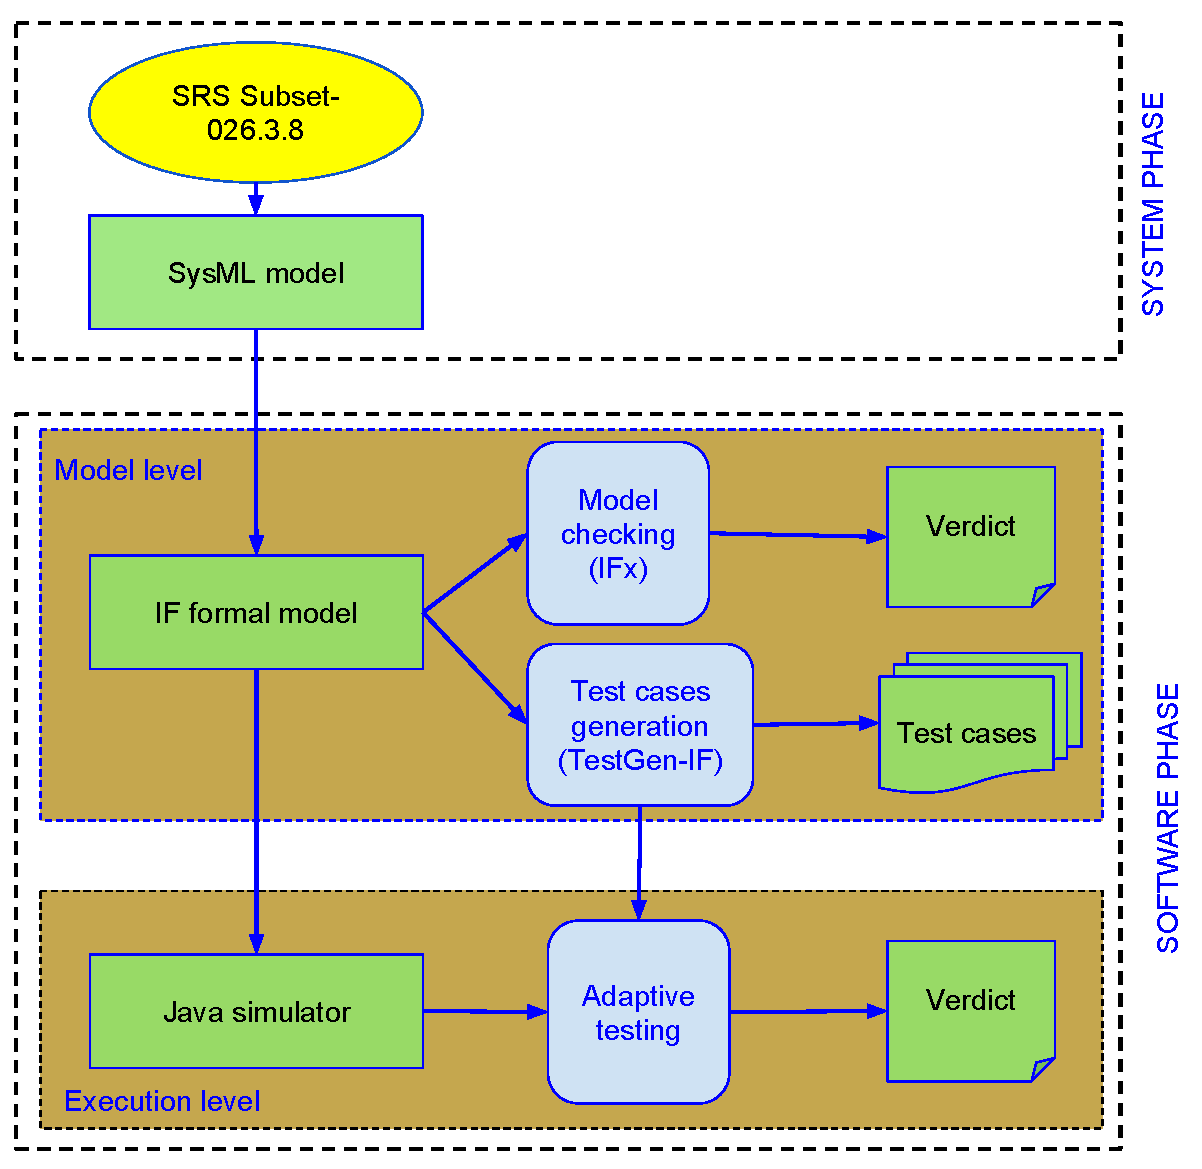
\includegraphics[width=.7\textwidth]{figures/TSP-approach.pdf}
  \caption{Overview of Institut Telecom-Mines' Approach}
  \label{fig:approach}
\end{center}
\end{figure}


In the openETCS project, the system requirement specifications are represented
by using SysML models. We validate and verify the models on two aspects,
model-level and execution-level, by using two model-based techniques:
model-checking and model-based testing.
%
Model checking is a technique for automatically verifying whether a model of a system meets some given safety requirement.
To solve such a problem, both the model of the system and the requirements are firstly formulated in some precise mathematical language.
Model checking algorithms are then used to check the model against the requirement.
Basically, all states of the model will be visited exhaustively to meeting the requirement or finding a counterexample. 
Model-based testing is a approach to test whether a system satisfies some requirements.
It executes some test cases delivered from the requirements on the system under test to give verdict.

At the model-level, V\&V is done through model-checking, by using IFx tool, of
IF formal models which are representations of the SysML models.
At the execution-level, we encode the SysML models by Java simulators that are
then used to execute some tests.
We also illustrate the consistency of two aspects by applying test cases, that
are generated by TestGen-IF tool at the model-level, on our Java simulators,
i.e., all tests must give {\em pass} verdict

The automatic translations from SysML models to IF models to Java simulators are
being studied. Furthermore, as the actual models provided by WP3 have not yet
been initiated, we started with a formal model that is a finite state machine
augmented with continuous variables and guards. This model can be considered as
an abstract version of ETCS model and it can be refined in our future steps,
e.g., the MOVE function mode of the TRAIN can be refined to SHUNTING,
TRIP function modes of OBU in Subset-026 chapter 4.4.

%%%%%%%%%%%%%%%%%%%%%%%%%%%%%%%%%%%%%%%%%%%%%%%%%%%%%%%%%%%%%%%%%%%%%%%%%%%%%%
\subsection{Verification on IF model}
\subsubsection{Object of Verification}
The object of verification is an IF model representing the Movement Authority of
the train.

\subsubsection{Available Specification}
The Movement Authority is described in Subset-026 chapter 3.8. This chapter
gives (1) the definitions and structure of the movement authority, 
(2) the procedures of OBU to send a Movement Authority request to
the RBC and to receive a Movement Authority response from the RBC;
and (3) the use of Movement Authority on the OBU.

%Chapter 4.4 of Subset-026 describes in detail 16 different movement modes of
% OBU such as ISOLATION, TRIP, STAND BY, \ldots. At the moment, we generalize these modes onto
%two abstract modes: MOVE and STOP specifying when the train are moving or not.

\subsubsection{Detailed Verification Plan}

\paragraph{Goal} 
We intend firstly to model the Movement Authority of OBU described in
Subset-026 chapter 3.8. We then use the model to validate the safety
properties and to generate the test.


\paragraph{Means}

We consider an ETFSM (Extended Timed Finite State Machine) as a formal model
from which test cases for verifying the safety aspects of the developed
implementations can be automatically generated.
Formally, 
    an ETFSM is a tuple 
    $(S, s_0, E, T,  \Delta, v_0)$ where:
    $S$ is a non-empty finite set of states with $s_0 \in S$ as the
        initial state,
 $E$ is a finite set of events,
 $T$ is a set of transitions, 
 $\Delta \subset S \to S \times (\mathbb{N} \cup \{ \infty \})$ is timeout function, and
 $\vec{v}_0$ is the vector of initial values of the context variables.
The timeout function $\Delta$ limits an interval by which a trigger of
transition must occur (thus the transition will be fired). 
When the interval ends, the transition will be automatically fired in spite of
its trigger has not yet occurred.
The figure~\ref{fig:model} represents the ETFSM model of the Movement Authority of OBU .

\begin{figure}[!htbp]
\begin{center}
  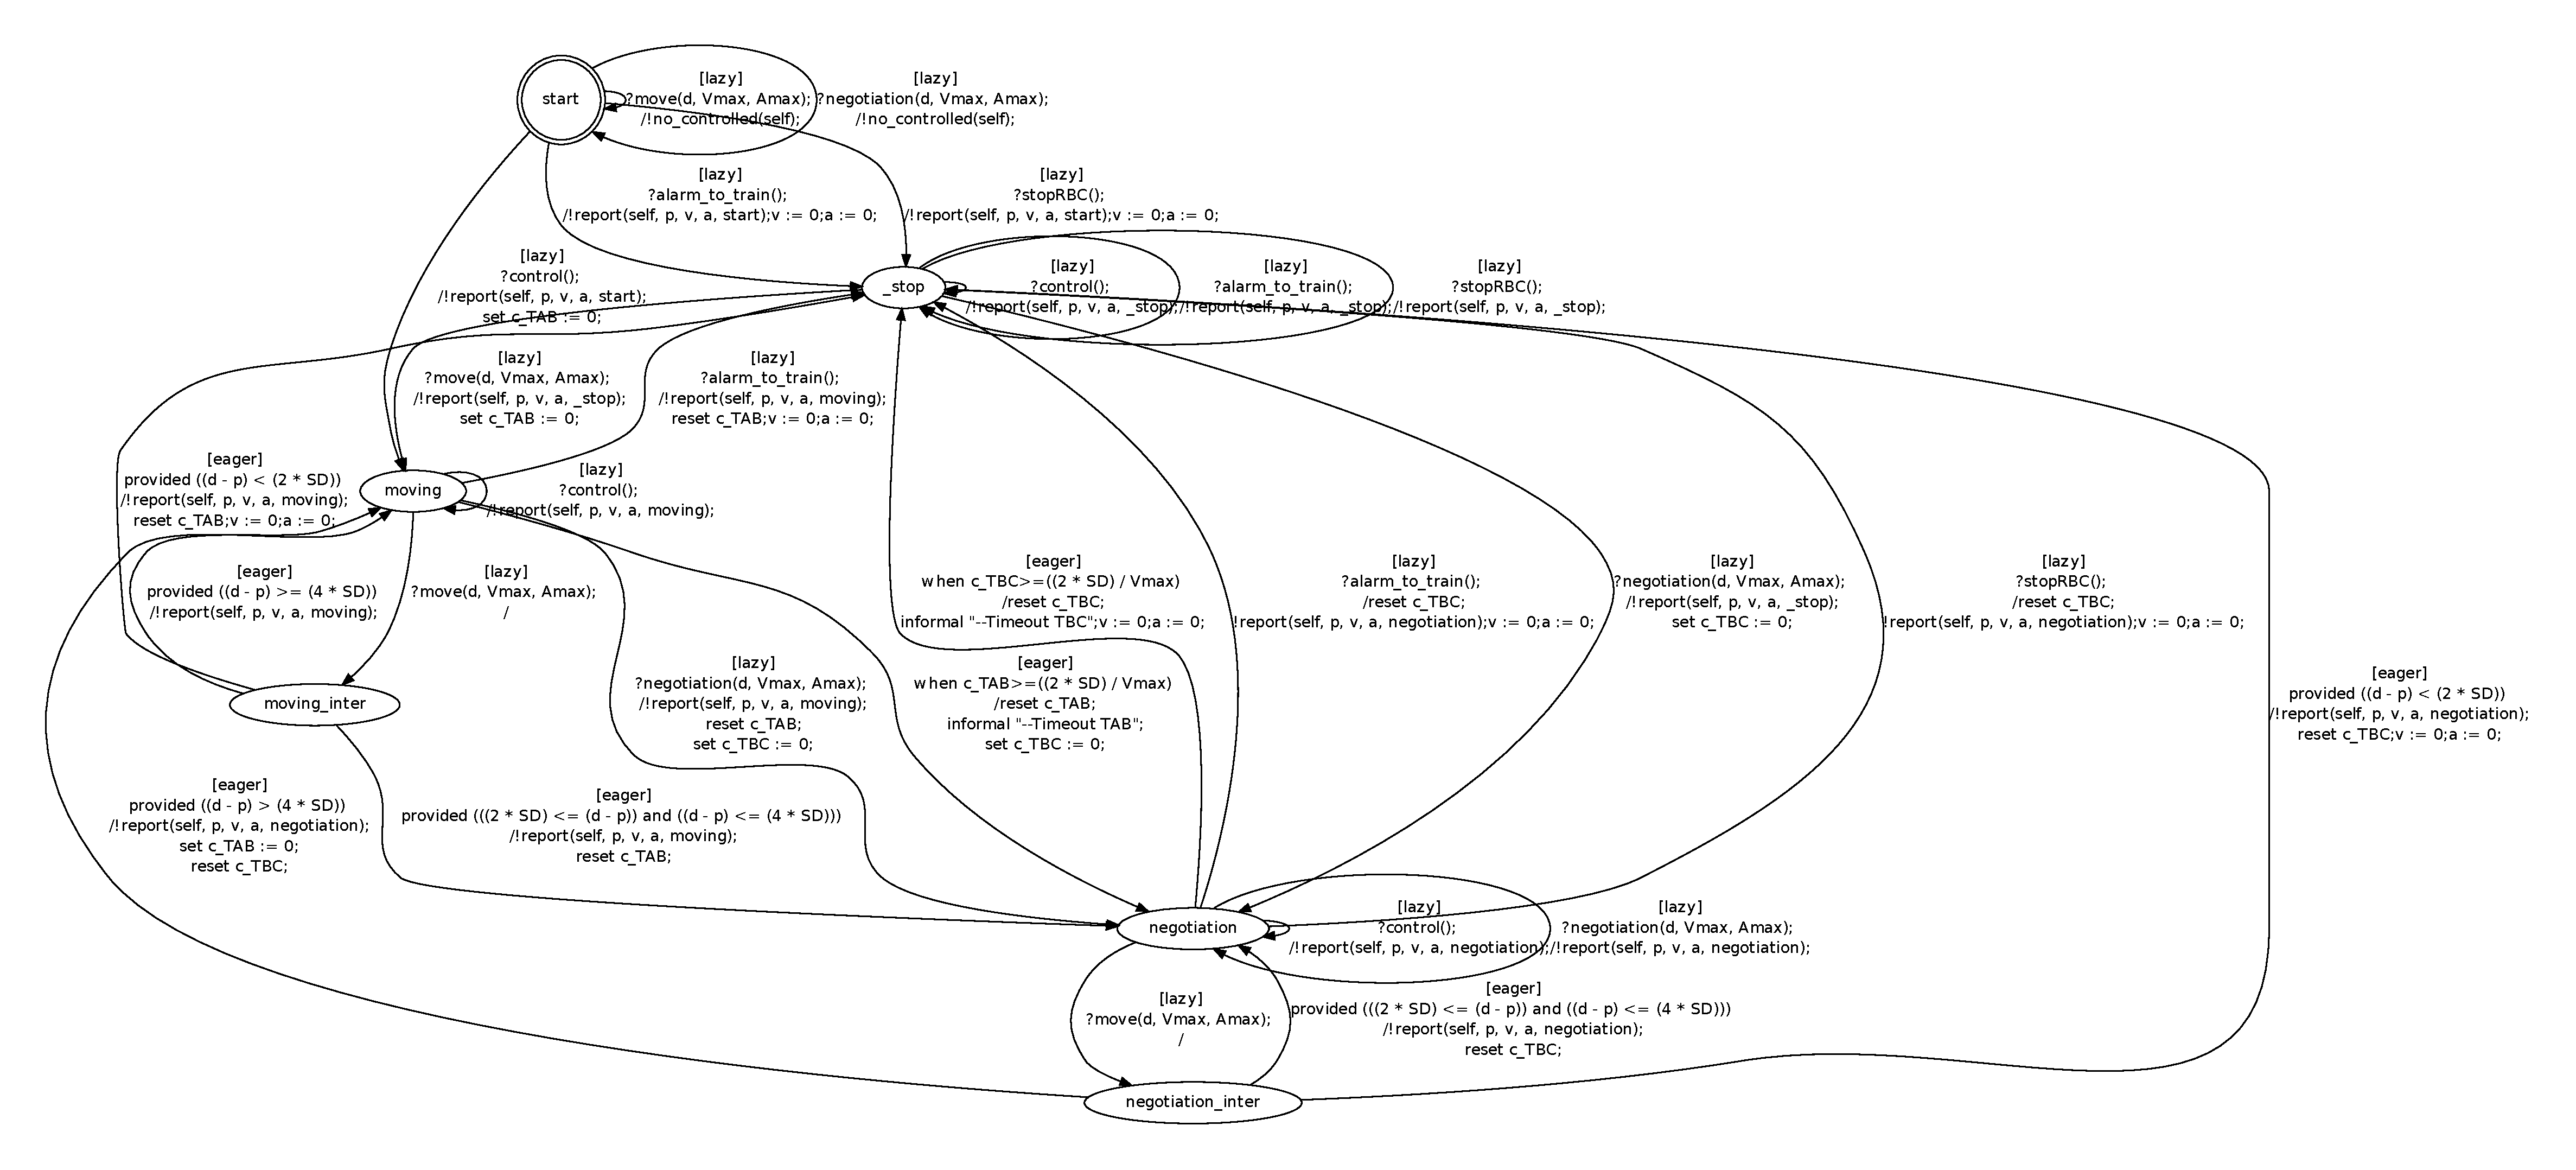
\includegraphics[width=24.5cm, angle=90]{figures/if-model.pdf}
  \caption{Extended Timed Finite State Machine of OBU}
  \label{fig:model}
\end{center}
\end{figure}

\paragraph{Method}


Model checking is an automatic technique for verifying finite-state reactive
systems. Using such techniques one could automatically check if the model
specifies most of the requirements of the system, such as the important safety
properties described in Task 4.4. Similar to proof techniques, in order to use
model checking to verify if the SFM (Semi-formal model) and FFM (fully formal
model) comply with the safety and function requirements,
the properties to be proven have to be identified and described. To implement
the use model checking, it is mandatory to specify the model using finite-state
reactive systems, and they should also provide an intuitive way to express the
properties to be model checked. The language for describing a formal model for
which corresponding model checkers exist should be selected and the set of
critical requirements to be verified need to be clearly identified. The proposed
model checking techniques should be supported in the selected tool chain. 

\paragraph{Tool}
We use IF mdoel-checker () for model-checking and 
TestGen-IF for generating test cases.
The formal model is hence represented by IF description% or XML 
in order to be checked by using IF model-checker.


\subsubsection{Results}



We have provided a method to formally model the
movement authority requirements of the train using
finite state machines augmented with continuous variables (train position, speed, acceleration) and
time constraints. 

We have modeled OBU on Timed Extended Finite State Machine.
We have then used IF model checker to verify the
proposed formal model. 

During the modeling we discovered 3 inconsistencies, ambiguities and gaps in the specification
which we reported in~\cite{specfindingsTSP}.

%\paragraph{Conclusions/Lessons Learned}

Currently, the obtained model can be considered as an abstract representation
of the system specification provided by the standard, i.e., the MOVE
function mode of the OBU can be refined to SHUNTING, TRIP function modes of
OBU in Subset-026 chapter 4.4.


\subsubsection{Next Steps}

On the one hand, we refine our formal model to take into account different
function modes of OBU.
In the other hand, we complete the automatic translations from the SysML
specification to the IF specification or to our Java simulator.

%%%%%%%%%%%%%%%%%%%%%%%%%%%%%%%%%%%%%%%%%%%%%%%%%%%%%%%%%%%%%%%%%%%%%%%%%%%%%%%%%
\subsection{Verification on Java simulator}

\subsubsection{Object of Verification}
Model of the Movement Authority converted from IF language to the simulator.

\subsubsection{Available Specification}
Conversion of the IF model described on the previous section.

\subsubsection{Detailed Verification Plan}

\paragraph{Goal} 
We intend firstly to model the Movement Authority of OBU described in
Subset-026 chapter 3.8. We then use the model to validate the safety
properties and to generate the test.

\paragraph{Means}


When using model checkers the criteria for the model to be safe is that all the
safety properties should be checked. This is impossible, since the number of
safety properties could be infinite and thus, only some of them can be checked
through the above step.
For this reason, as a complementary approach, testing is commonly used. If the
corresponding model respects some requirements, i.e., only expected outputs are
produced to applied input sequences, to some extent, there is a confidence that
the models is safe. In order to derive ‘good’ tests a formal model should be
involved. It is known that only the FSM model where each input is followed by a
corresponding output allows automatic deriving finite tests with the guaranteed
fault coverage where the races between inputs and outputs can be easily avoided.
 Many authors for deriving finite tests with the guaranteed fault coverage turn
their model to some kind of an FSM (see,
e.g.,~\cite{springintveld2001testing,zymc11,Gromov2009}).

We decided to use TestGen-IF to automatically extract a set of test cases from
the formal model described in the IF language. We have identified a set of basic
requirements and we can describe them as IF properties.  Based on these
properties, the TestGen-IF tool automatically generates a set of test cases.
TestGen-IF implements Hit-or-Jump~\cite{Cavallib} algorithm stategry to generate the test.
These test cases can be used to test if the model follows the requirements defined for the test generation.


For simulation, the artifacts should provide means to execute the model.  The
simulator must be automatically generated, so that, when run against test
scenarios (inputs/outputs for the model), we may conclude whether the model
follows the specification or not. In particular, it is important to define test
scenarios for the safety critical properties. The simulation should cover all states,
transitions, data-flow, and paths in the model. It would also be desirable to
include graphical representation of the simulation/model and also provide a
report of the visited components. Being able to trace the
requirements that are met during a simulation is also advisable to allow simple
requirement coverage.

Once we have a test suite generated by TestGen-IF, we execute them using our simulator. The simulator provides a trace of the execution of each test and the expected trace. By comparing both traces it is possible to identify problems with the model.


\subsubsection{Results}


We have provided a method to formally model the
requirements of the ETCS using finite state machines
augmented with continuous variables (train position, speed, acceleration) and
time constraints. 

We have modeled OBU on TEFSM.
With TestGen-IF we automatically generated a test suite that was used to verify our simulator.
%


By providing TestGen-IF with test objectives, we were able to automatically generate a test suite capable of verifying the properties related to them. Currently we have four different test objectives and with them we generated a suite of 22 tests. By providing more test objectives it is possible to generate more tests.
Each test constitutes a sequence of inputs (or period of time without an input) and expected outputs.

The tests generated were executed by the simulator. When executing a test, the simulator provides a file that compares the expected trace generated from the model with the trace that was generated by the simulator. If an inconsistency occurs, the test is considered failed. On our first execution we found some inconsistencies between the IF model and the model used by the simulator. After taking care of these inconsistencies we were able to execute all the tests pass.

It is possible to find inconsistencies in a model using the Java simulator to execute tests. However, further testing is needed to determine the completeness of our test suite.

\subsubsection{Next Steps}
We plan to verify the fault coverage of these tests by executing Java
simulator against corresponding traces and Java Mutants. For this stage we used an older version of the model. A newer version is currently being updated and will be used on future activities.